
\documentclass[a4paper,11pt]{article}

\usepackage{amsmath,amssymb,amsfonts,amsthm}    % Typical maths resource packages
\usepackage{graphicx}                           % Packages to allow inclusion of graphics
\usepackage{hyperref}                           % For creating hyperlinks in cross references
\usepackage[authoryear]{natbib}                 % literature reference style
\usepackage[bf]{caption2}

\usepackage[utf8]{inputenc}
\usepackage[T1]{fontenc}
\usepackage[english]{babel}
\usepackage{listings}
\usepackage{xcolor}
\usepackage{eso-pic}
\usepackage{mathrsfs}
\usepackage{url}
\usepackage{amssymb}
\usepackage{amsmath}
\usepackage{multirow}
\usepackage{hyperref}
\usepackage{booktabs}
\usepackage{tikz}
\usepackage{lvblisting}
\usepackage{cooltooltips}
\usepackage{colordef}
\usepackage{float}

% -------------------------------
% --- some layout definitions ---
% -------------------------------

% define topline
\usepackage[automark]{scrpage2}
\pagestyle{scrheadings}
\automark{section}
\clearscrheadings
\ohead{\headmark}

% define citation style
\bibliographystyle{ecta}

% define page size, margin size
\setlength{\headheight}{1.1\baselineskip}
\voffset=-2cm
\hoffset=-3cm
\textheight24cm
\textwidth15.5cm
\topmargin1cm
\oddsidemargin3cm
\evensidemargin3cm

% define line line spacing = 1.5
\renewcommand{\baselinestretch}{1.5}

% define second level for `itemizing'
\renewcommand{\labelitemii}{-}




% --------------------------------------
% --------------------------------------
% --------------------------------------
% --- the structure the tex document ---
% ---  (this our recommendation) -------
% frontmatter:
%   - titlepage (mandatory),
%   - acknowledgement,
%   - abstract,
%   - table of contents (mandatory),
%   - list of abbreviations (not mandatory),
%   - list of figures (not mandatory),
%   - list of tables  (not mandatory) .
%
% body of the thesis (the structure of the thesis body is not mandatory, but the list of literature is mandatory):
%   - introduction,
%   - methods,
%   - data,
%   - results,
%   - conclusion,
%   - literature (mandatory),
%   - appendix (figures, tables).
%
% last page:
%   - declaration of authorship (mandatory).
% --------------------------------------
% --------------------------------------
% --------------------------------------

\begin{document}

% -------------------------------
% --- frontmatter: Title page ---
% -------------------------------

\thispagestyle{empty}
\begin{center}

    {\Large{\bf Bachelor's/Master's Thesis Title}} \vspace{0.5cm}


    {\normalsize Bachelor's/Master's Thesis submitted\\\vspace{0.5cm}
    to}\\\vspace{0.5cm}
    {\normalsize{\bf Prof. Dr. Nikolaus Hautsch}} \\\vspace{0.5cm}
    {\normalsize Humboldt-Universit\"at zu Berlin \\
    School of Business and Economics \\
    Institute for Statistics and Econometrics \\
    Chair of Econometrics} \vspace{1cm}


    {\normalsize by \\\vspace{0.5cm}
    {\bf your name} \\
    (your matriculation number)} \vspace{1cm}


    {\normalsize in partial fulfillment of the requirements \\
    for the degree of \\
    {\bf Bachelor/Master of Science} \\
    Berlin, September 30, 2007}

\end{center}




% -----------------------------
% --- frontmatter: Contents ---
% -----------------------------
\newpage
\tableofcontents
\clearpage


% ----------------------------------------------------
% --- frontmatter: List of Abbreviations (not mandatory) ---
% ----------------------------------------------------
\newpage
\addcontentsline{toc}{section}{List of Abbreviations}
\ohead[]{LIST OF ABBREVIATIONS}
\section*{List of Abbreviations}

\begin{tabular}{rp{0.2cm}lp{1cm}rp{0.2cm}l}
    CPI     & &  Consumer Price Index   & & ETF     & &  Equity Traded Funds  \\
    ETH     & &  Eat the Horse          & & XLM     & &  Xetra Liquidity
\end{tabular}




% ----------------------------------------------------
% --- frontmatter: List of Figures (not mandatory) ---
% ----------------------------------------------------
\newpage
\addcontentsline{toc}{section}{List of Figures}
\ohead[]{\rightmark}
\listoffigures



% ---------------------------------------------------
% --- frontmatter: List of Tables (not mandatory) ---
% ---------------------------------------------------
\newpage
\addcontentsline{toc}{section}{List of Tables}
\listoftables



% -------------------------------
% --- main body of the thesis ---
% -------------------------------
\newpage
\pagestyle{plain}
\setcounter{page}{1}    % start page numbering anew
\pagenumbering{arabic}  % page numbers in arabic style


\section{Introduction}

Airbnb (airbnb.com) is now a famous website allowing private people and commercial entities to rent out part of their spaces. It all started in 2007 when two 27-year-olds decided to sublet their living room in their San Francisco apartment during a conference to help pay their rent \citep{airbnbstory:2012}. Now, they are a multibillion-dollar company where properties from all over the world are on rent \citep{businessinsider}.

Many studies have already been conducted on price determinants for the hotel industry, like the ones named in \cite{wang2017price}, and for Airbnb properties \cite{wang2017price} itself, but none so far specific for the city of Berlin. We therefore attempted an exploratory analysis of Airbnb listings in Berlin and, in particular, of their price. For this purpose linear regression on price was also run and properties were clustered.

As in \cite{wang2017price} summarized, in the case of hotels, hotel prices are negatively influenced by the hotel's location, since shorter distance from the city center, the main attractions and/or important transportation points leads to higher prices. On the other side positive influences on price are hotels'star rating and online customer rating, the services and amenities provided, and by the "presense of car parks and fitness centers". But price determinants could be different in case of different types of accomodations, such as the ones offered on Airbnb. That's why \cite{wang2017price} also derived the drivers of price for Airbnb listings from 33 cities.

What is observed is that the dimension as well as the type of the accomodation positively influences the price. However, the location has almost no impact on the price, except for the case of being inside the circulare with respect to the opposite. Clustering on the other hand did not deliver usable results,  because of the absence of easily recognizable patterns. Further analysis of the price determinans and the clusters may shed more light into the topic.


The paper is divided into 7 sections. Section \ref{Sec:Data Preparation} will present the data used for this study and explained how it was prepared. Consecutively, \ref{Sec:Exploratory} will run exploratory data analysis, both in form of tables and plots, on this data. Because of our interest in explaining property price, \ref{Sec:Price analysis} will focus on this feature and show correlation and regression with respect to it. Furthermore, an attempt at clustering the Airbnb properties will be done in \ref{Sec:cluster}. After that it will be explained in \ref{Sec:shiny} why a ShinyApp was develop to present this research. Finally, \ref{Sec:Conc} we will present the results and draw some conclusions.

\newpage
\section{Data}\label{Sec:Data}

For the analysis explained in this paper data was downloaded for a website independent from airbnb itself. insideairbnb (\href{http://insideairbnb.com/}{insideairbnb.com}) scrapes (????) airbnb to get its data and posts it online for the public to use on own analysis, while also providing some analysis of its own.
\\
The data is divided according to cities and for each there is general information about the city's properties and their availability for the next year. The variables that are being kept for this analysis are listing on table 1. (HOW TO MAKE IT CHANGE NUMBER???).



\section{Method/Model/Theory}\label{Sec:Method}

\begin{itemize}

    \item How was the data analyzed ?

    \item Present the underlying economic model/theory and
        give reasons why it is suitable to answer the given problem.

    \item Present econometric/statistical estimation method and
        give reasons why it is suitable to answer the given problem.

    \item Allows the reader to judge the validity of the study and
        its findings.

    \item Depending on the topic this section can also be split up
        into separate sections.

\end{itemize}

\newpage
\section{Results}\label{Sec:Results}

\begin{itemize}

    \item Organize material and present results.

    \item Use tables, figures (but prefer visual presentation):
        \begin{itemize}
            \item Tables and figures should supplement (and not duplicate) the
                text.

            \item Tables and figures should be provided with
            legends.\\
                {\it Figure \ref{Fig:Resids} shows how to include and reference
                graphics. The graphic must be labelled before. Files must be in
                \texttt{.eps} format.}

                \begin{figure}[ht]
                \begin{center}
                    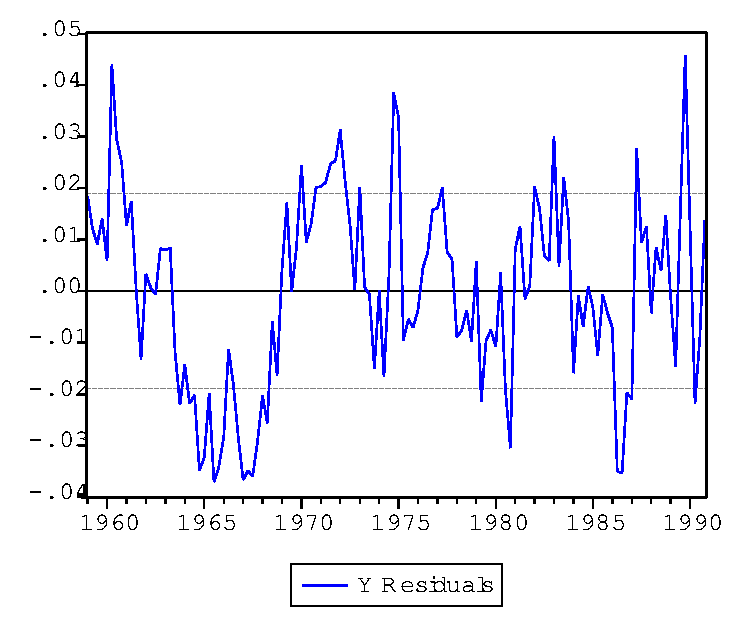
\includegraphics[scale=0.5,angle=0]{graph}
                    \caption{Estimated residuals from model XXX. ...}
                    \label{Fig:Resids}
                \end{center}
                \end{figure}

            \item Tables and graphics may appear in the text or in
                the appendix, especially if there are many simulation results
                tabulated, but is also depends on the study and number of tables resp.
                figures. The key graphs and tables must appear in
                the text!
        \end{itemize}

    \item Latex is really good at rendering formulas:\\
        {\it Equation (\ref{Eq:SpecDens}) represents the ACs of a stationary
        stochastic process:
        \begin{equation}
            f_y(\lambda) = (2\pi)^{-1} \sum_{j=-\infty}^{\infty}
                           \gamma_j e^{-i\lambda j}
                         =(2\pi)^{-1}\left(\gamma_0 + 2 \sum_{j=1}^{\infty}
        \gamma_j \cos(\lambda j)\right)
                                        \label{Eq:SpecDens}
        \end{equation}
        where $i=\sqrt{-1}$ is the imaginary unit, $\lambda \in [-\pi,
        \pi]$ is the frequency and the $\gamma_j$ are the autocovariances
        of $y_t$.}

\newpage

    \item Discuss results:
        \begin{itemize}
            \item Do the results support or do they contradict economic theory ?
            \item What does the reader learn from the results?
            \item Try to give an intuition for your results.
            \item Provide robustness checks.
            \item Compare to previous research.
        \end{itemize}
\end{itemize}

\section{Results and Conclusions}\label{Sec:Conc}

\begin{itemize}

    \item Give a short summary of what has been done and what has been
    found.

    \item Expose results concisely.

    \item Draw conclusions about the problem studied. What are the
    implications of your findings?

    \item Point out some limitations of study (assist reader in judging validity
    of findings).

    \item Suggest issues for future research.

\end{itemize}




% ----------------
% --- appendix ---
% ----------------
\appendix

% literature
\newpage
\addcontentsline{toc}{section}{References}
\bibliography{literature}



% --------------------------------------------
% --- last page: Declaration of Authorship ---
% --------------------------------------------

\newpage
\thispagestyle{empty}
%{\Large{\bf Declaration of Authorship}}\vspace{0.5cm}

\section*{Declaration of Authorship}

I hereby confirm that I have authored this seminar paper independently and without use of others than the indicated
sources. All passages which are literally or in general matter
taken out of publications or other sources are marked as such.
\vspace{1cm}

Berlin, \today \vspace{0.5cm}

Silvia Ventoruzzo



\end{document}
